\documentclass[tikz,crop,preview, border=1cm, landscape]{standalone}

\def\meanOne{0.8}
\def\meanTwo{0.4}
\def\binOne{0.7}
\def\binTwo{0.22}
\def\binTwoDev{0.1}
\usepackage{tikz}
\usepackage{pgfplots}

\begin{document}
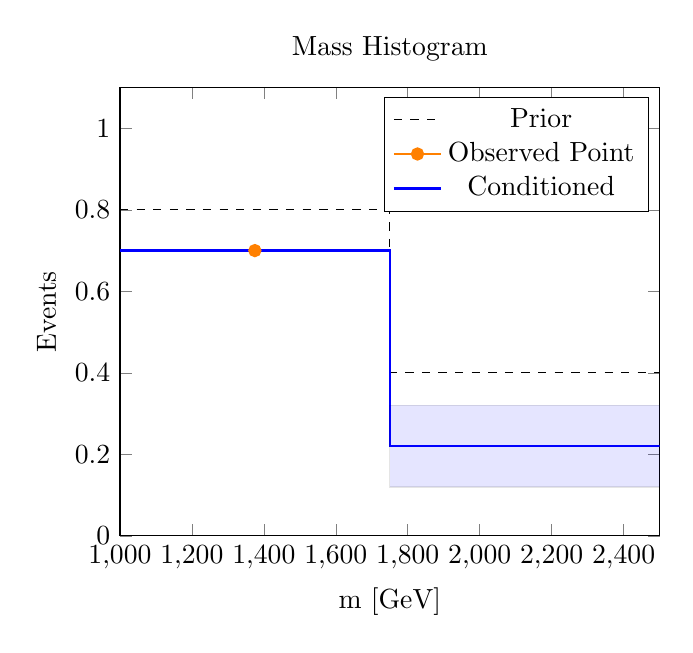
\begin{tikzpicture}
  \def\center{(axis cs: \meanOne,\meanTwo)}
  \begin{scope}
    \begin{axis}[
      ymin=0, ymax=1.1,
      xmin=1000, xmax=2500,
      xlabel={m [GeV]},
      ylabel={Events},
      title=Mass Histogram,
      ]
      \addplot[dashed, black, const plot mark mid, domain=1000:2500, samples=2, mark=none] plot coordinates {(1000,\meanOne) (2500,\meanTwo)};
      \addplot[orange, thick, mark=*] plot coordinates {(1375,\binOne)};
      \addplot[blue, thick, const plot mark mid, domain=1000:2500, samples=2, mark=none] plot coordinates {(1000,\binOne) (2500,\binTwo)};
      \draw[fill=blue, opacity=0.1] (axis cs:1750,\binTwo-\binTwoDev) rectangle (axis cs:2500,\binTwo+\binTwoDev);
      \legend{Prior, Observed Point, Conditioned}
    \end{axis}
  \end{scope}
\end{tikzpicture}
\end{document}
